\section{Directed Graphs}

\epigraph{\emph{I mean, if 10 years from now, when you are doing
something quick and dirty, you suddenly visualize that I am looking over
your shoulders and say to yourself ``Dijkstra would not have liked
this,'' well, that would be enough immortality for me.}}{%
---Edsger W.\xspace Dijkstra}

\noindent A graph is a data structure $G = \langle V, E \rangle$ where
$V = \{ v_0, \ldots, v_n \}$ is the set of vertices (or nodes) and $E =
\left \{ \langle v_i,v_j \rangle, \ldots \right \}$ is the set of edges
that connect the vertices. For example, you might have a set of cities
$V = \{ \text{El Cajon}, \text{La Mesa}, \text{San Diego}, \ldots,
\text{La Jolla} \}$ as the vertices and write ``El Cajon'' $\rightarrow$
``Lakeside'' to indicate that there is a path (Los Coches Road) from El
Cajon to Lakeside. If there is a path from El Cajon to Lakeside, as well
as a path from Lakeside to El Cajon, then the edge connecting El Cajon
and Lakeside is \emph{undirected}.

% \begin{wrapfigure}{r}{0.145\textwidth}
% \centering
%   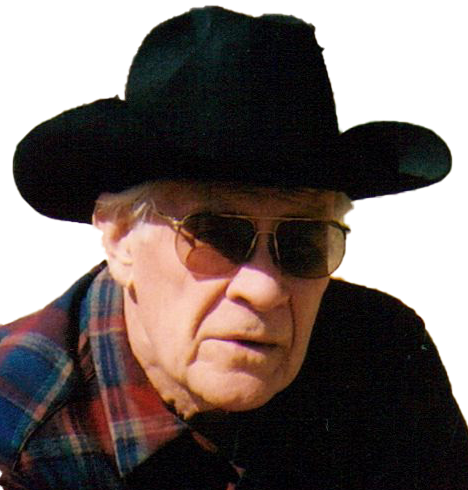
\includegraphics[width=0.14\textwidth]{images/DDL-blk.png}
% \end{wrapfigure}

Such a simple graph representation simply tells you how vertices are
connected and provides the idea of one-way roads. But it really does not
help Denver, since it does not provide any notion of distance. We solve
this problem by associating a weight with each edge and so we might
write ``Santee $\rightarrow$ El Cajon, 2'' to indicate that there is a
path of two miles long from Santee to El Cajon. Given a set of edges and
weights, then we can then find the shortest path from any vertex to any
other vertex (the answer may be that there is no such path). There are
elegant (and quick) algorithms for computing the shortest path, but that
is not exactly what we want to do. We want to find a path through all
of the vertices, visiting each \emph{exactly once}, such that there is a
direct (single step) connection from the last vertex to the first. This
is called a \emph{Hamiltonian path}. This will address Denver's need to
get home, but won't necessarily be the shortest such path. So, we need
to go through every possible Hamiltonian path given the list of cities
Denver is traveling through and pick the shortest path. Note: if you
find yourself on a path that is longer than the current best found
Hamiltonian path, then you can preemptively reject your current path.

\section{Representing Graphs}

\epigraphwidth=0.65\textwidth
\epigraph{\emph{We live on a placid island of ignorance in the midst of
black seas of infinity, and it was not meant that we should voyage
far.}}{---H.\xspace P.\xspace Lovecraft, \emph{The Call of Cthulhu}}

\noindent Perhaps the simplest way to represent a graph is with an
\emph{adjacency matrix}. Consider an $n \times n$ adjacency matrix $M$,
where $n$ is the number of vertices in the graph. If $M_{i,j} = k$,
where $1 \le i \le j \le n$, then we say that there exists a
\emph{directed edge} from vertex $i$ to vertex $j$ with weight $k$.
Traveling through wormholes is considered hazardous, so any valid edge
weight $k$ must be non-zero and positive.

\begin{center}
\begin{blockarray}{ccccccccc}
 & 0 & 1 & 2 & 3 & 4 & 5 & $\dotsi$ & 25\\
\begin{block}{c[>{\medspace}cccccccc<{\medspace}]}
    0 & 0 & 10 & 0 & 0 & 0 & 0 & 0 & 0 \\
    1 & 0 & 0 & 2 & 5 & 0 & 0 & 0 & 0 \\
    2 & 0 & 0 & 0 & 0 & 0 & 3 & 0 & 5 \\
    3 & 0 & 0 & 0 & 0 & 21 & 0 & 0 & 0 \\
    4 & 0 & 0 & 0 & 0 & 0 & 0 & 0 & 0 \\
    5 & 0 & 0 & 0 & 0 & 0 & 0 & 0 & 0 \\
    \smash{\vdots} & 0 & 0 & 0 & 0 & 0 & 0 & 0 & 0 \\
    25 & 0 & 0 & 0 & 0 & 0 & 0 & 0 & 0 \\
\end{block}
\end{blockarray}
\end{center}

\newcommand{\edge}[3]{\langle #1,#2,#3 \rangle}

\noindent Each edge will be represented as a triple $\edge{i}{j}{k}$. The set of
edges in the adjacency matrix above is
\[
E = \left \{
  \edge{0}{1}{10},
  \edge{1}{2}{2},
  \edge{1}{3}{5},
  \edge{2}{5}{3},
  \edge{2}{25}{5},
  \edge{3}{4}{21}
\right \}.
\]

\noindent If the above adjacency matrix were made to be \emph{undirected}, it
would be reflected along the diagonal.

\begin{center}
\begin{blockarray}{ccccccccc}
 & 0 & 1 & 2 & 3 & 4 & 5 & $\dotsi$ & 25\\
\begin{block}{c[>{\medspace}cccccccc<{\medspace}]}
    0 & 0 & 10 & 0 & 0 & 0 & 0 & 0 & 0 \\
    1 & 10 & 0 & 2 & 5 & 0 & 0 & 0 & 0 \\
    2 & 0 & 2 & 0 & 0 & 0 & 3 & 0 & 5 \\
    3 & 0 & 5 & 0 & 0 & 21 & 0 & 0 & 0 \\
    4 & 0 & 0 & 0 & 21 & 0 & 0 & 0 & 0 \\
    5 & 0 & 0 & 3 & 0 & 0 & 0 & 0 & 0 \\
    \smash{\vdots} & 0 & 0 & 0 & 0 & 0 & 0 & 0 & 0 \\
    25 & 0 & 0 & 5 & 0 & 0 & 0 & 0 & 0 \\
\end{block}
\end{blockarray}
\end{center}

\noindent The first of the ADTs you will need to implement for this
assignment is for the graph. An \textbf{ADT} is an \emph{abstract data
type}. With any ADT comes an interface comprised of \emph{constructor},
\emph{destructor}, \emph{accessor}, and \emph{manipulator} functions.

\begin{clisting}{}
struct Graph {
    uint32_t vertices;                   // Number of vertices.
    bool undirected;                     // Undirected graph?
    bool visited[VERTICES];              // Where have we gone?
    uint32_t matrix[VERTICES][VERTICES]; // Adjacency matrix.
};
\end{clisting}

We elect to use an adjacency matrix with set maximum dimensions. This is
both to simplify the abstraction and also due to the computational
complexity of solving the Traveling Salesman Problem (TSP) with
depth-first search (DFS), which is discussed in \S 5. The
\texttt{VERTICES} macro will be defined and supplied to you in
\texttt{vertices.h}. In this header file, there is another macro
\texttt{START\_VERTEX} which defines the origin vertex of the shortest
Hamiltonian path we will be searching for. \textcolor{red}{You may not
modify this file. The \texttt{struct} definition of a graph \emph{must}
go in \texttt{graph.c}.}
\begin{clisting}{\texttt{vertices.h}}
#pragma once

#define START_VERTEX 0   // Starting (origin) vertex.
#define VERTICES     26  // Maximum vertices in graph.
\end{clisting}

The interface for the graph ADT is defined as
follows:

\begin{funcdoc}{Graph *graph\_create(uint32\_t vertices, bool undirected)}
  The constructor for a graph. A constructor function is responsible for
  initializing and allocating any memory required for the type it is
  constructing. It is through this constructor in which a graph can be
  specified to be undirected. Make sure each cell of the adjacency
  matrix, \texttt{matrix}, is set to zero. Also make sure that each
  index of the \texttt{visited} array is initialized as \texttt{false}
  to reflect that no vertex has been visited yet. The \texttt{vertices}
  field reflects the number of vertices in the graph. A working
  constructor for a graph is provided below. Note that it uses
  \texttt{calloc()} for \emph{dynamic memory allocation}. This function
  is included in \texttt{<stdlib.h>}.

  \begin{clisting}{}
Graph *graph_create(uint32_t vertices, bool undirected) {
    Graph *G = (Graph *)calloc(1, sizeof(Graph));
    G->vertices = vertices;
    G->undirected = undirected;
    return G;
}
  \end{clisting}

\end{funcdoc}

\begin{funcdoc}{void graph\_delete(Graph **G)}
  The destructor for a graph. A working destructor for a \texttt{Graph}
  is provided below. Any memory that is allocated using one of
  \texttt{malloc()}, \texttt{realloc()}, or \texttt{calloc()}
  \emph{must} be freed using the \texttt{free()} function. The job of
  the destructor is to free all the memory allocated by the constructor.
  \textcolor{red}{Your programs are expected to be free of memory
  leaks.} A pointer to a pointer is used as the parameter because we
  want to avoid \emph{use-after-free} errors. A use-after-free error
  occurs when a program uses a pointer that points to freed memory. To
  avoid this, we pass the \emph{address of a pointer} to the destructor
  function. By \emph{dereferencing} this double pointer, we can make
  sure that the pointer that pointed to allocated memory is updated to
  be \texttt{NULL}.

  \begin{clisting}{}
void graph_delete(Graph **G) {
    free(*G);
    *G = NULL;
    return;
}
  \end{clisting}
\end{funcdoc}

\begin{funcdoc}{uint32\_t graph\_vertices(Graph *G)}
  Since we will be using \texttt{typedef} to create \emph{opaque} data
  types, we need functions to access fields of a data type. These
  functions are called \emph{accessor} functions. An opaque data type
  means that users do not need to know its implementation outside of the
  implementation itself. This also means that it is incorrect to write
  \texttt{G->vertices} outside of \texttt{graph.c} since it violates
  opacity. This accessor function returns the number of vertices in the
  graph.
\end{funcdoc}

\begin{funcdoc}{bool graph\_add\_edge(Graph *G, uint32\_t i, uint32\_t j, uint32\_t k)}
  The need for \emph{manipulator} functions follows the rationale behind
  the need for accessor functions: there needs to be some way to alter
  fields of a data type.

  This function adds an edge of weight \texttt{k}
  from vertex \texttt{i} to vertex \texttt{j}. If the graph is
  undirected, add an edge, also with weight \texttt{k} from \texttt{j}
  to \texttt{i}. Return \texttt{true} if both vertices are within bounds
  and the edge(s) are successfully added and \texttt{false} otherwise.
\end{funcdoc}

\begin{funcdoc}{bool graph\_has\_edge(Graph *G, uint32\_t i, uint32\_t j)}
  Return \texttt{true} if vertices \texttt{i} and \texttt{j} are within
  bounds and there exists an edge from \texttt{i} to \texttt{j}. Remember:
  an edge exists if it has a non-zero, positive weight. Return
  \texttt{false} otherwise.
\end{funcdoc}

\begin{funcdoc}{uint32\_t graph\_edge\_weight(Graph *G, uint32\_t i, uint32\_t j)}
  Return the weight of the edge from vertex \texttt{i} to vertex
  \texttt{j}. If either \texttt{i} or \texttt{j} aren't within bounds, or
  if an edge doesn't exist, return 0.
\end{funcdoc}

\begin{funcdoc}{bool graph\_visited(Graph *G, uint32\_t v)}
  Return \texttt{true} if vertex \texttt{v} has been visited and
  \texttt{false} otherwise.
\end{funcdoc}

\begin{funcdoc}{void graph\_mark\_visited(Graph *G, uint32\_t v)}
  If vertex \texttt{v} is within bounds, mark \texttt{v} as visited.
\end{funcdoc}

\begin{funcdoc}{void graph\_mark\_unvisited(Graph *G, uint32\_t v)}
  If vertex \texttt{v} is within bounds, mark \texttt{v} as unvisited.
\end{funcdoc}

\begin{funcdoc}{void graph\_print(Graph *G)}
  A debug function you will want to write to make sure your graph ADT
  works as expected.
\end{funcdoc}
